\chapter{KB-Specific Network(KBSN)}
\section{知识库概述}
人类智能体通过学习和实践不断获取知识与经验,并能将习得的知识存储在记忆系统中,面对相关问题时能准确、快速地调用相关的知识和经验,完成识别和推理过程,成功解决问题。人工智能系统的终极目标便是能像人类一般快速、准确地解决未知问题,甚至超越人类的物理极限,实现范围更广、更艰深的任务解决。人类在真实世界中的学习是不断将非结构化的信息重构为结构化的知识的过程,知识库(KB)是一种包含常识和描述真实世界的事实的知识集,在不同的应用情景中有不同的内部结构。

知识库最早被应用于人工智能中的专家系统\citing{akerkar2010knowledge},专家系统是一种建立在知识库基础上,使用推理方法完成复杂推理过程,最终实现与人类专家同水平的决策能力的计算机系统,被广泛应用于医学诊断、分子结构推理、自然语言理解等领域。专家系统面向的专家任务需要特定领域的知识,这也使得知识库成为专家系统的核心之一。针对不同领域的任务构建知识的表达方式是困难的,因为专家知识可能是不精确的,同时要从知识库中获取答案的过程依赖于人工的制定复杂的规则,知识库精度和人力成本等因素制约了专家系统在更多领域的应用。

知识库也被应用于在自然语言处理的任务,例如机器翻译和文本问答。知识库中的本体包含某个领域中的各种概念和概念间的关系,本体在机器翻译中可作为知识源\citing{nirenburg1994machine}。语言学中的多义词在不同的语境中被解释为不同的含义,人类能根据上下文语境的不同选择出最恰当的词语,但对于机器翻译系统便是一大难题。当机器翻译系统能够获得足够多的本体作为知识源时,能较好地解决多义词的解释问题,从而得到更加准确的翻译结果\citing{knight1993building}。

文本问答系统在早期作为专家系统的交互界面,在之后的发展中逐渐独立出来成为自然语言处理的一个分支,文本问答系统根据给出的文本问题,从文本知识库中提取答案,此时的文本知识库往往是文本组成的文档,还未使用资源描述框架(RDF)的结构化数据。大多数文本问答系统都采用相对标准的结构:根据问题文本建立查询、利用信息提取方法(IR)确定可能包含答案的文章位置、进一步确定答案所在的片段,这种架构下不使用任何与答案相关的额外知识\citing{hermjakob2000knowledge}。Hermjakob等人提出了将手写规则和概念本体相结合的问答系统——Webclopedia\citing{hermjakob2000knowledge}。Webclopedia由对输入问题进行句法和语义的解析的问题解析模块、用于文档查询的查询模块、用于获得与答案相关的文档的信息提取模块、片段解析模块、答案匹配模块和答案生成模块构成。系统在多个模块中使用了知识库提高精确度,在问题解析过程中使用了语言知识库——由30000个节点的概念层级、140个问题/答案类型和词库组成,帮助系统确定问题的句法结构;在查询模块中使用了WordNet\citing{miller1995wordnet}扩展与问题关键词关联的信息;在答案匹配模块中也使用了常识和事实知识库,系统的架构如图\ref{Webclopedia}。
\begin{figure}[H]
	\centering
	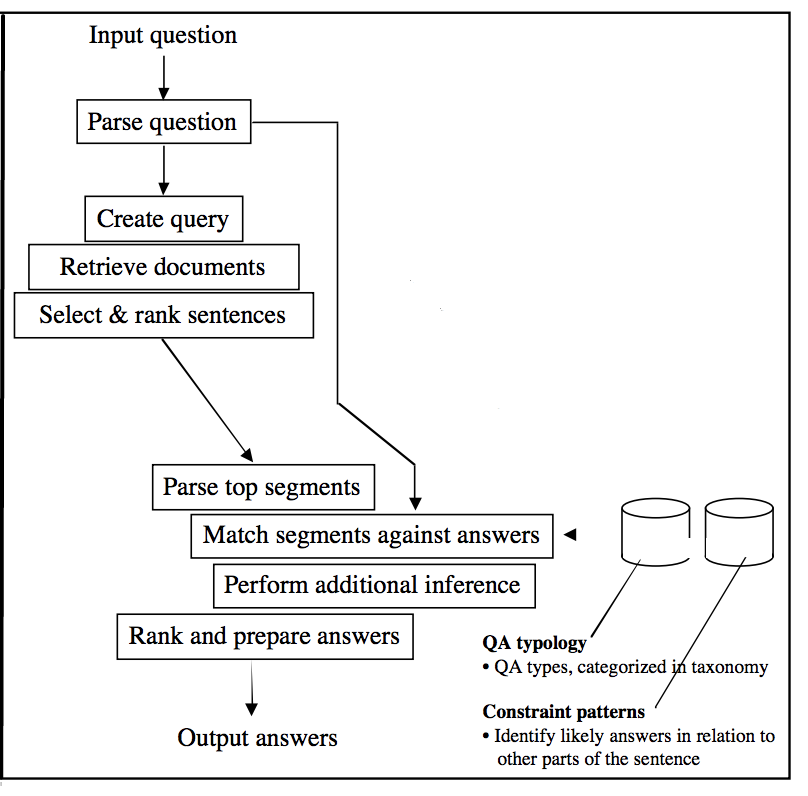
\includegraphics[width=0.8\textwidth]{Webclopedia.png}
	\caption{Webclopedia系统架构}
	\label{Webclopedia}
\end{figure}

应用信息提取技术(IR)的问答系统有一个非常明显的缺点——只能根据问题确定答案相关的文章或者段落,不能给出更为直接的答案。为解决这种缺陷,研究人员探索了更多的方法。

Burke等人一改通常的从文章中提取答案的方式,先将被频繁问到的问题(FAQ)以“问题-答案”对的形式存储为知识库,再从新问题中寻找与知识库匹配程度最高的“问题-答案”对,进而获得答案\citing{burke1997question}。在此方法中最核心的步骤是对新旧问题之间的匹配,为了使匹配的问题之间的语义相似度最大,系统还使用了WordNet\citing{miller1995wordnet}的语义知识,WordNet能提供词语和其同义词集合、同义词集合之间的关系,因此能避免一些匹配过程中的歧义错误,提高匹配的准确度。这里以“匹配”为核心思想的算法最大的障碍是常见问题集的容量、深度和广度问题,因此通常对于范围较小的场景而言,才能实现较好的匹配准确度。Rinaldi等人提出一个专门针对技术领域的基于知识的问答系统ExtrAns\citing{rinaldi2002towards}。ExtrAns以技术手册为知识库,将问题文本和知识库都转化为一种称为“最小逻辑形式”(MLF)的语义表达,并通过逻辑证明提取出答案。

随着资源描述框架(RDF)在构建知识库的兴起,知识库也由原来的文档形式转化为冗余更小、可扩展性更强、易用性更强的结构化数据库。面对由于互联网技术的普及带来的海量网页、文章、超文本、图片等多种模态的资源,研究者们对信息的整合进行了探索\citing{smith1981multibase,wiederhold1993intelligent,subrahmanian1994amalgamating,embley1998ontology,alani2003automatic},语义网和相关技术的出现促进了大尺度知识库的发展,出现了DBpedia\citing{auer2007dbpedia}、OpenIE\citing{banko2007open}、Yago\citing{suchanek2007yago}、Freebase\citing{bollacker2008freebase}、Wikidata\citing{vrandevcic2014wikidata}等多种含有常识和特定领域知识的知识库,这些配置灵活、结构统一且语义丰富的外源知识库也促进了基于知识库的视觉问答方法的兴起。

\begin{comment}
\section{常见的知识库}
知识表达是人工智能中历史较为悠久的领域,并且大量的知识表达模型被提出,从最早的“框架和脚本”(frame and script)\citing{minsky1974framework,schank2013scripts}到后来的逻辑表达方式、资源描述框架(RDF)和网络本体语言(OWL)。随着互联网技术的普及,海量的网页、文章、超文本、图片等多种模态的资源被创造,如何将这些海量松散的多模数据重组为结构化的数据成为计算机科学的重要任务之一,大量的研究对信息的整合进行了探索\citing{smith1981multibase,wiederhold1993intelligent,subrahmanian1994amalgamating,embley1998ontology,alani2003automatic},语义网和相关技术的出现促进了大尺度知识库的发展,出现了DBpedia\citing{auer2007dbpedia}、OpenIE\citing{banko2007open}、Yago\citing{suchanek2007yago}、Freebase\citing{bollacker2008freebase}、Wikidata\citing{vrandevcic2014wikidata}等多种含有常识和特定领域知识的知识库。

除了知识库以外还有一种常用的存储数据的方式——数据库。数据库通常被组织成表格的方式,表内使用数值或者字符的方式表示数据,首行罗列出不同的属性,其余行则代表存储的数据。数据库中的表与表之间存在的指针代表表之间的联系。不同于数据库,知识库不以表为组织形式,而是由大量形式为(主语,谓语,宾语)的三元组构成的图结构,这样的三元组以资源描述框架(RDF)为模型基础\citing{lassila1997resource},能够方便的通过查询语句获得信息。“主语”和“宾语”表示知识库中的实体,“谓语”代表两者之间的关系。例如,将“猫种类属于哺乳类”转化的三元组形式为(猫,种类属于,哺乳类),“猫”是主语,“种类属于”是谓语,“哺乳类”是宾语。数据库与知识库的结构对比如图\ref{db-kb}。
\begin{figure}[H]
	\centering
	\subfigure[数据库的表结构]{
		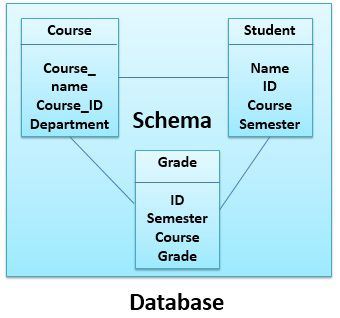
\includegraphics[width=0.5\textwidth]{database.jpg}}
	\subfigure[知识库的由三元组构成的图结构]{
		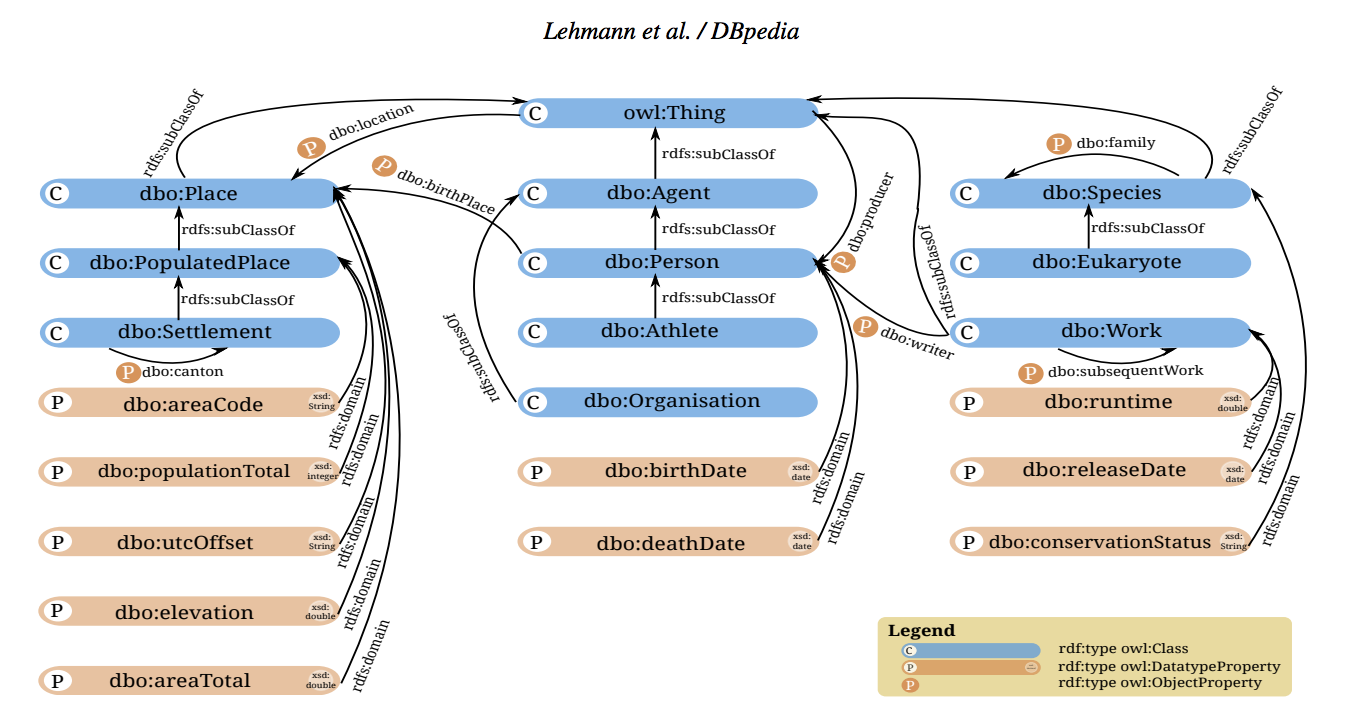
\includegraphics[width=0.7\textwidth]{kb.png}}
	\caption{数据库与知识库不同的数据组织形式}
	\label{db-kb}
\end{figure}

知识库具有高通用性、高可读性的特征。通过资源描述框架(RDF)能将所有现实中可描述的事物和事物间的关系组织到知识库中,这种通用性特征能够极大地提高了自动化系统存储、交换和使用信息;三元组的结构来源于语言学中“主谓宾”的基本语句构成方式,这既符合人类的认知方式,也是一种简单的数据组织形式,因此高可读性即使针对人类可读也是针对机器可读。正是因为知识库是建立在真实世界事实的描述之上,因此它能成为复杂决策和推理的基石,从人类推理过程看,知识库便是复杂推理的“起点”。
\end{comment}

\textbf{Yago}
知识库通常由人工和自动化提取两种方式构建得到,对比这两种不同构建方式,自动化提取的知识库往往质量较低,容易包含错误信息,而人工构建的知识库能满足较高的精度要求,但由于人工构建的成本较高,因此此类知识库有数据容量受限、构建周期长、内容老化快等缺陷。

Suchanek等人结合Wikipedia文章的广博性和WordNet优秀的语义分类,提出了自动化生成本体的知识库YAGO\citing{suchanek2007yago}。Wikipedia的文章对某个话题或概念进行详细的多角度说明,同时大多数文章都归属于一个或者多个类别,类别页面既包含了大量实体和概念,可以作为知识库中的本体,同时类别页面也隐含着概念之间的平行关系和所属关系,这能提供一定的结构关系。YAGO利用Wikipedia目录页面提取出其中的实体和实体之间的关系,同时结合WordNet中概念的清晰层次关系,实现了97\%的准确率。初始版本中涉及90万个实体和500万个实体之间的关系。

YAGO被设计为可扩展的知识库,能够结合特定领域的知识源或是从网络上提取得到的信息构建领域相关的知识库,因此之后的研究者也在此基础上进行了多种的扩展。YAGO2在YAGO基础上引入GeoNames——包含超过700万个地点信息,在“实体-关联”的表示方法中加入了时间和空间维度,不仅能丰富事实的准确性,还能反应出实体在时空层面的变化\citing{hoffart2013yago2}。YAGO3构建了一个多语言的知识库\citing{mahdisoltani2013yago3}。

\textbf{DBpedia}
Wikipedia是由非盈利组织维基媒体基金会(Wikimedia Foundation)构建的世界上最大的多语言的开放性网络百科全书,其通过文章的形式对词条进行多方面的介绍,文章中包含大量的结构化信息,例如文字、信息框模板、分类信息、图片、地理坐标信息、超链接等,这些多模态的信息能丰富知识的多样性,并且建立知识的关联。但作为网络应用,Wikipedia的搜索能力和其他网络应用一样,只能满足关键词的搜索,这种状况大大的降低了知识之间的关联和价值,同时因为其作为大规模协同性内容编辑平台,文章内容也难以避免的出现数据矛盾、不一致的分类和错误。

Auer等人为了充分挖掘Wikipedia中已有的人类知识,并构建知识结构,提出了DBpedia知识库\citing{auer2007dbpedia}。Wikipedia为实现统一的文章风格,因此在文章编辑中镶嵌了一些信息框模板,如图\ref{dbpedia}。
\begin{figure}[h]
	\centering
	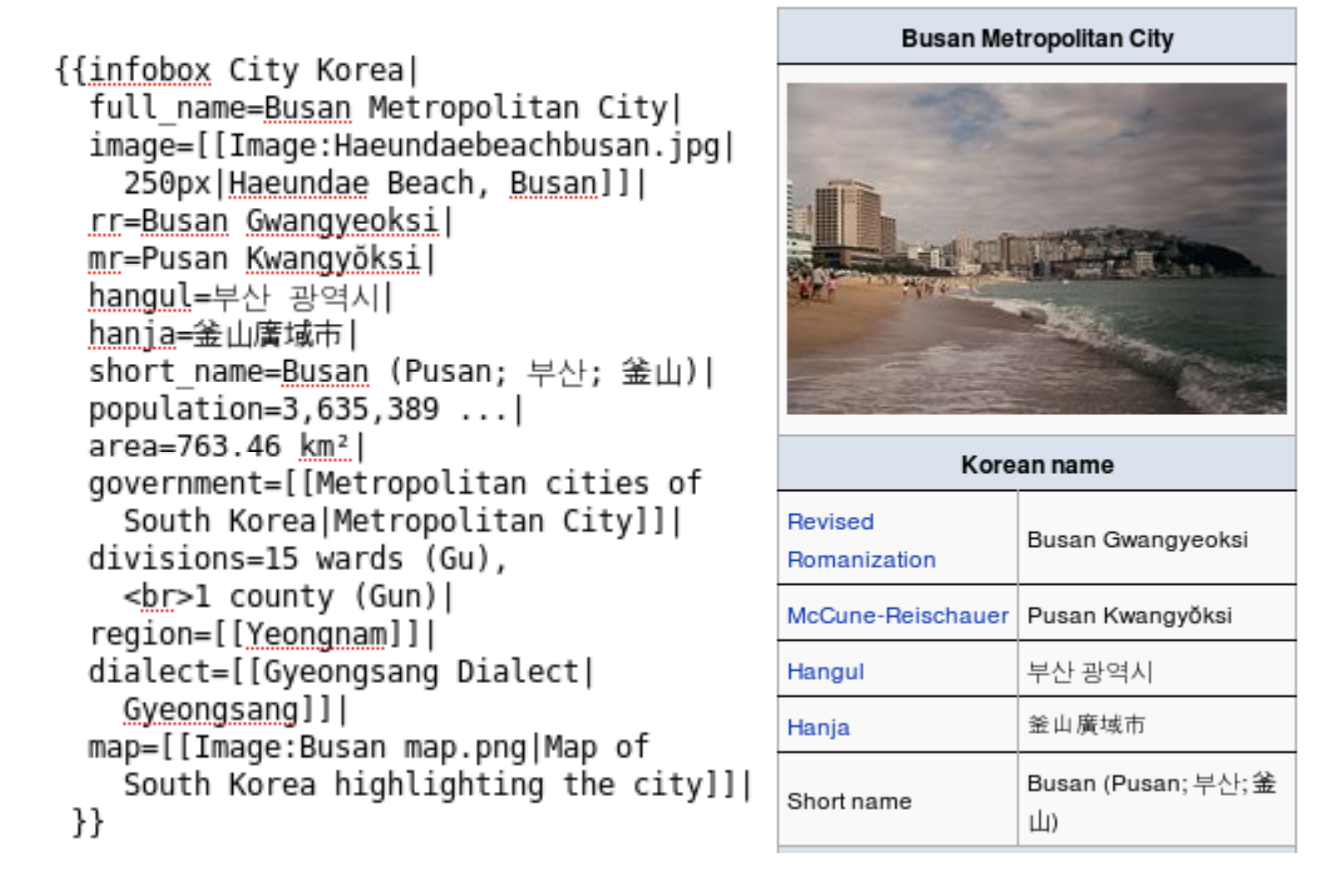
\includegraphics[width=0.8\textwidth]{dbpedia.png}
	\caption{Wikipedia的信息框模板和加载效果}
	\label{dbpedia}
\end{figure}
DBpedia利用信息框提取算法检测信息框模板,并且提取出关键的信息,再将信息转化为资源描述框架(RDF)的三元组结构,从而将Wikipedia的文章内容转化为机器可读的结构化信息。最初版本的DBpedia知识库包含关于195万实体的信息,实体内容包括人物、地点、音乐专辑和电影,除了实体外还包含65.7万个图片链接、160万个外部网页链接、18万个其他资源描述框架(RDF)数据库、20.7万个Wikipedia目录和7.5万个YAGO类别\citing{suchanek2007yago}。随着开放社区的数据丰富,2016年推出的版本中已经包含6600万实体,实体的类型扩充了视频、游戏、组织、物种和疾病\citing{wikipedia2016}。资源描述框架的三元组数据量也从1亿增长到130亿之多。

为了增强DBpedia的数据易用性,Auer等人提供了三种数据获取方式:链接数据、SPARQL协议和可下载的RDF文件。链接数据通过HTTP协议获取发布与互联网上的RDF数据,提供给语义网络浏览器、语义网路爬虫和语义网络查询客户端访问\citing{timlinked}。SPARQL是专门针对资源描述框架的查询语言,通过SPARQL终端向\url{http://dbpedia.org/sparql}发送查询指令,DBpedia知识库会返回相应的查询结果。可下载的RDF文件包含序列化的RDF三元组数据,DBpedia将整个数据库按照数据的类型分为众多子数据集,例如,文章目录集、目录标签集、地理坐标集、图像集等。

知识库的内容多样性、易用性和大体量为DBpedia应用提供了良好的基础设施,因此一些自然语言问答和交互的应用都选择建立在DBpedia丰富的知识之上。NLI-GO DBpedia是一个针对通用自然语言交互的应用程序,程序可以接受自然语言问题,并通过SPARQL查询DBpedia知识库,给出答案,实际上这就是基于DBpedia的文本问答系统\citing{nli-go},类似的还有款基于DBpedia的聊天机器人——DBpedia Chatbot。许多基于知识库的视觉问答研究也选择了数据更加准确的DBpedia\citing{wang2015explicit,wang2017fvqa,wu2016ask}。

\textbf{OpenIE}
应用于构建知识库的信息提取技术(IR)往往需要人为构建大量手写规则,并选择合适的语料库,当已有的提取模型面对全新领域的语料库时,需要重新编写提取规则或者标注数据,这种系统在面对快速迭代和具有丰富多样性的互联网数据时,便会遇到自动化程度低、语料库异质性和效率问题。

为了节省信息提取过程的自动化程度,并能大范围应用于不同领域,Banko等人提出了一种能自主学习不同语料库的信息提取模型——开放信息提取技术(Open IE)\citing{banko2007open}。Open IE以语料库为输入,通过内部算法对语料库中的语句进行一次遍历,最终提取出语句中蕴含的(实体,关系,实体)三元组数据,在整个过程中不需要人工参与,因此可以应用于不同领域知识库的构建。

Banko等人还提出了一种应用高扩展性Open IE模型的系统TEXTRUNNER。TEXTRUNNER由自监督学习器、单通道提取器、基于冗余的评估器三个主要模块构成。自监督学习器以小的语料样本作为训练集,首先使用语句解析器从样本中粗略地提取出(实体,关系,实体)的三元组数据,再对提取出的内容进行标注,标注为“可信”和“不可信”两种标签,将带有标签的数据作为朴素贝叶斯分类器的训练样本。提取器遍历整个语料库,提取出所有可能的三元组数据。对于同一个句子,提取器能生成一个或多个三元组数据,这些数据将被送入学习器训练得到的分类器中,保留所有分在“可信”类别的数据。在得到所有提取出的知识后,评估器融合相同的数据,计算不同的数据的数量。基于以上统计,评估器对每一个三元组数据分配一个用于判断知识正确性的概率值,其中的假设是,如果从多个的语句中提取出相同的知识,那么该知识拥有较高的可信度。

在实验阶段,TEXTRUNNER从包含1.3亿个句子的900万个网页中提取出6000万个三元组数据,平均每个句子提取出2.2个关系数据。通过数据过滤、随机抽取、人工判定等方式,作者对提取数据的完整性和正确性进行了概率评估,过滤后的数据包含1130万个三元组数据,其中780万的数据被评估为“格式正确”且概率标签在0.8以上,80.4\%“格式正确”的数据通过人工评估被认定为正确的,从实体间的关系看,“格式正确”的数据中反映抽象事实的占86\%,其中77.2\%是正确的;反映具体事实的占14\%,其中88.1\%是正确的,如图所示\ref{textrunner}。
\begin{figure}[H]
	\centering
	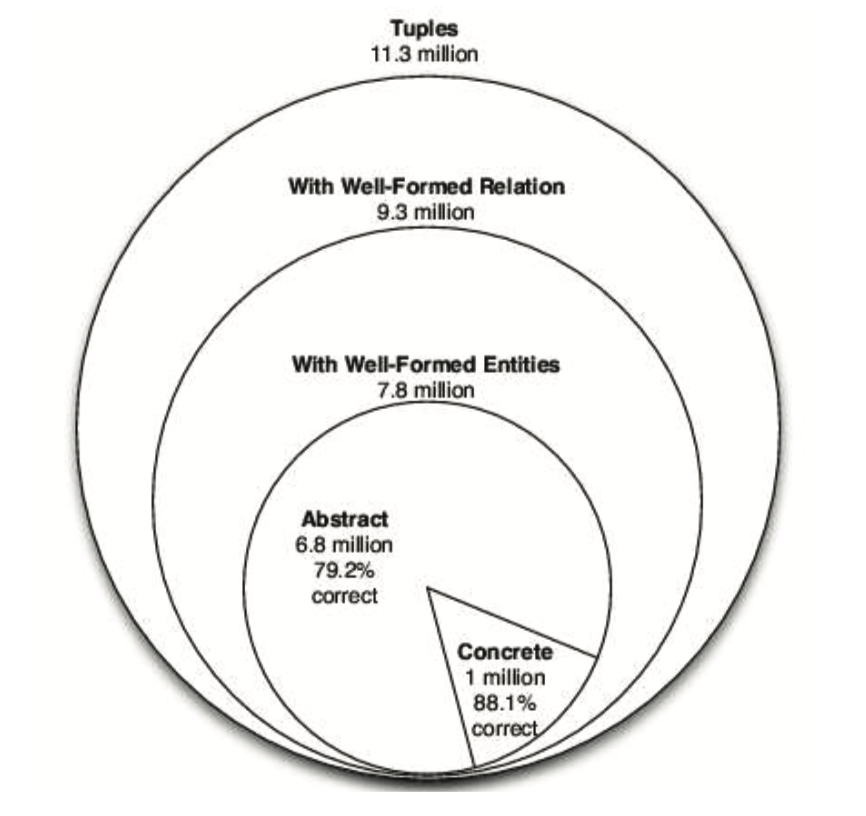
\includegraphics[width=0.5\textwidth]{textrunner.png}
	\caption{TEXTRUNNER在实验环境下知识提取的正确率}
	\label{textrunner}
\end{figure}

Wu等人在TEXTRUNNER的基础上提出了WOE开放信息提取系统\citing{wu2010open}。WOE改进了自监督学习方式用于构建提取器,TEXTRUNNER在提取过程中使用解析器直接从语料库中提取(实体,关系,实体)的三元组数据,而WOE则先从Wikipedia的信息框中提取“属性-值”对,再使用匹配器从文章中找到包含文章主语和“属性-值”对的句子作为语料库中的训练数据。随后测试了两种解析方法的提取器:WOE-parse和WOE-pos,WOE-pos使用和TEXTRUNNER类似的解析方法,根据简单的词性标签,从语料库中的句子解析出(实体,关系,实体)的数据,WOE-parse则选择更复杂的依赖解析树,希望能再复杂长句的解析中得到更好的精确度。

开放信息提取系统会对每个输出的三元组数据给定一个置信度,如果给定一个置信度的下限,高置信度的数据被保留,低置信度的数据被过滤,此时可以通过精确度和召回率测试系统的性能。精确度是指保留的数据中正确的数据所占比例,能反映整体精确度的平均水平。召回率是指保留的数据中正确的数据占所有正确数据的比例,能反映正确的数据在不同置信度的分布情况。

实验分析显示,因为使用了更友好的训练数据,WOE-pos在精确度上更优于TEXTRUNNER,而WOE-parse在解析树的帮助下实现了最好的性能,特别是在召回率上。

Fader等人在分析TEXTRUNNER和WOE的结果之后发现,不连贯提取和无信息提取两种错误频繁出现。不连贯提取是指被提取的关系语句由多词组成,但语义不连贯而无意义。无信息提取是指提取内容忽略了句子的关键信息,例如,“父亲对母亲做出承诺”,系统返回无信息的(父亲,做出,承诺)而不是(父亲,做出承诺对,母亲)。以上的两种错误都是由系统不能提取出具有完整句法结构的关系语句造成的,Fader等人在Open IE系统中引入了一定的句法限制,提出了REVERB开放信息提取系统\citing{fader2011identifying}。30\%的REVERB提取数据的概率标签在0.8或更高,相较起TEXTRUNNER的0.13\%,在精确度上实现了越阶式的增长,不连贯提取和无信息提取的错误率也大幅减少。

\textbf{Freebase}
Bollacker等人试图结合一般数据库的扩展和Wikipedia等百科全书的多样性,提出了Freebase数据库\citing{bollacker2008freebase}。Freebase和其他常用的知识库相同,使用资源描述框架的三元组形式结构化真实世界的知识,但同时继承了网络百科全书的开放和协同的思想,所有的内容创造和维护都由社区成员协作完成。Freebase存储的元组数据超过1亿2500万条,超过4000种类型和7000种属性,允许使用查询语言通过HTTP协议获取数据。

2014年,Google宣布关停Freebase并将数据迁移至Wikidata。

\textbf{Wikidata}
Wikidata是为了更高效地开放使用和管理Wikipedia文章中数据而提出的协同知识库\citing{vrandevcic2014wikidata}。由于Wikidata的出发点是希望通过大规模协同的方式构建知识库,因此Wikidata的数据具有开放性、多版本共存、多语言、易用性和持续更新的特性。Wikidata向所有用户提供数据扩展和编辑的权限;Wikidata为保证模糊数据的存疑性,相互之间有冲突的数据被同时展示;考虑到数字、日期、坐标等语言无关的数据内容,Wikidata与Wikipedia相同设计为多语言版本;Wikidata数据被组织成Json、RDF的形式发布于网络,通过网络服务能够轻松获取数据;社区成员的持续更新能保持Wikidata的时效性。

Wikidata数据的基本单元被称为项目(Item),每个项目包含名称标签、“Q+数字“的项目编码、描述、别名、和声明。声明中包含一系列属性和相应的值,用于详细描述项目的特点,项目页面如图\ref{wiki-item}。
\begin{figure}[H]
	\centering
	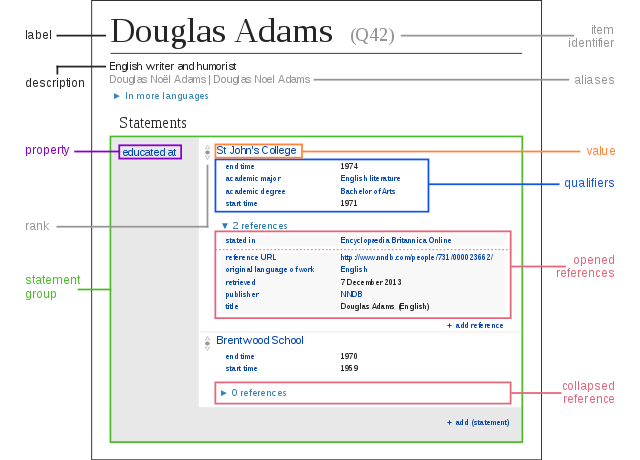
\includegraphics[width=0.8\textwidth]{wiki-item.png}
	\caption{wikidata项目页面}
	\label{wiki-item}
\end{figure}
项目之间通过有向无环图的方式构成,节点代表项目,有向线段代表项目之间的关系,如图\ref{wiki-dag}。截止到2018年,Wikidata已拥有超过5000万个项目。
\begin{figure}[H]
	\centering
	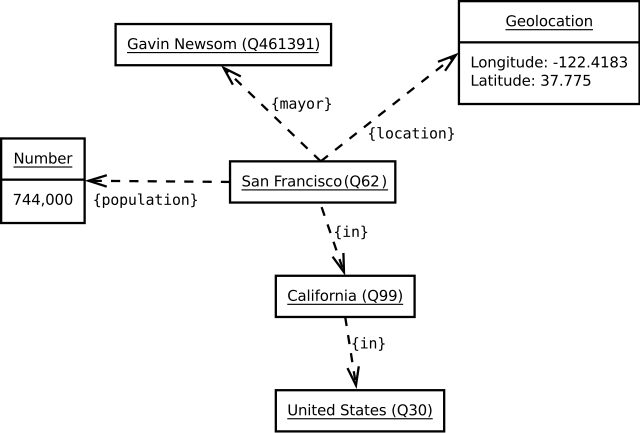
\includegraphics[width=0.8\textwidth]{wiki-dag.png}
	\caption{wikidata项目之间的有向无环图结构}
	\label{wiki-dag}
\end{figure}

Wikidata于2012年提出,相较起以往的知识库,开放性更强,限制也更少。对比YAGO和DBpedia,Wikidata不是从Wikipedia的目录或者信息框中提取信息,相反Wikidata被社区成员独立构建,并为Wikipedia作为知识源,数据被链接到Wikipedia文章中。对比Freebase将对象按类型划分的方式,Wikidata支持对所有对象赋予任意属性。

\section{KBSN的模型架构}

\section{实验}
\subsection{数据集}
\subsection{实验结果分析}

\section{结论}
